\section{Interface PWM}
Le module de PWM permet de contrôler un moteur grâce à une modulation par largeur d'impulsion(Pulse Width Modulation). Ce module prends en entrée un valeur sur 8bits permettant de régler la valeur
du rapport cyclique de la PWM.

Afin de créer un signal PWM, il a fallu coder un programme qui incrémente un compteur tout les cycles d'horloge puis met la sortie à l'état haut tant que le compteur est 
inféreur à la valeur du rapport cyclique. Lorsque le compteur dépasse la valeur du rapport cyclique, la sortie passe à l'état bas jusqu'à ce que le compteur arrive à 255. A ce
moment là, le compteur repasse à 0 et on recommence.

Ci dessous, une image d'une PWM avec un rapport cyclique de 33\%, la valeur en entrée est de 77.

\begin{figure}[h]
\centering
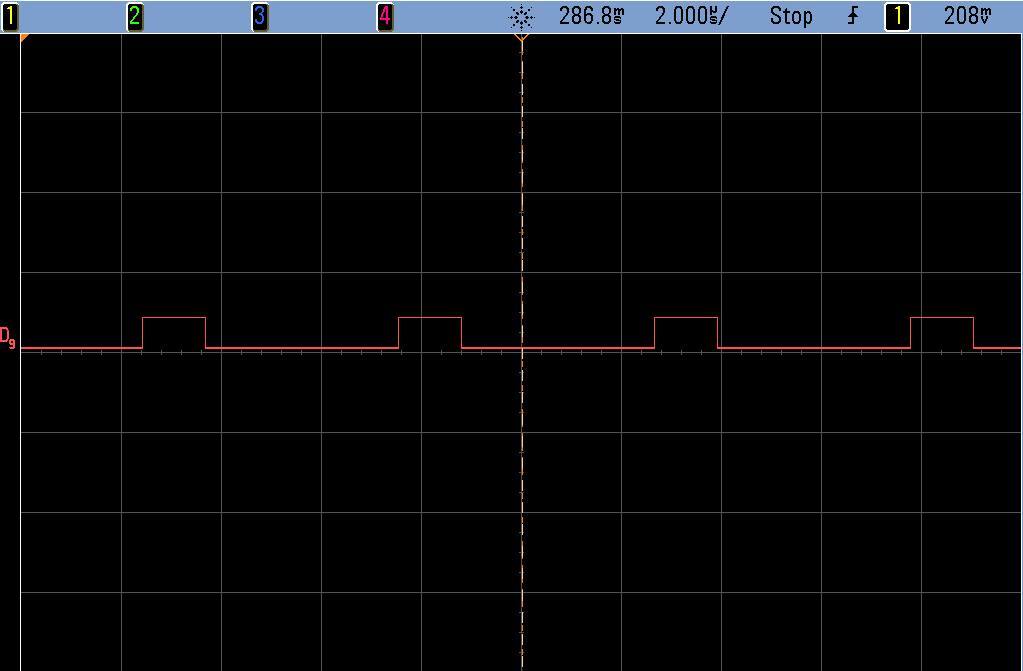
\includegraphics[width=10cm]{img/PWM_3F.png}
\caption{Exemple de signal PWM}
\end{figure}

Le code de la PWM est le suivant : 
\lstinputlisting[caption={Pwm.vhd},firstline=37]{../../../Pwm/src/Pwm.Vhd}

\pagebreak

